\documentclass{article}
\usepackage{iclr2027_conference,times}

\input{math_commands.tex}

\usepackage{hyperref}
\usepackage{url}
\usepackage{graphicx}
\usepackage{booktabs}
\usepackage{amsmath}
\usepackage{amssymb}
\usepackage{xcolor}
\usepackage{multirow}
\usepackage{wrapfig}
\usepackage{capt-of}
\usepackage[most]{tcolorbox}

% The ordering names are \texttt and do not hyphenate, so a line packed with
% them can overrun the margin; let TeX stretch the spaces instead.
\emergencystretch=1.5em

% Tighter float separation: the page budget is 9 pages of main text.
\setlength{\textfloatsep}{11pt plus 2pt minus 2pt}
\setlength{\floatsep}{9pt plus 2pt minus 2pt}
\setlength{\intextsep}{9pt plus 2pt minus 2pt}

% Finding box: one boxed claim per result-bearing section (package-free).
\definecolor{findingframe}{RGB}{38,148,132}
\definecolor{findingback}{RGB}{233,247,244}
\newsavebox{\findingbox}
\newenvironment{finding}
  {\par\smallskip\noindent\setlength{\fboxrule}{0.9pt}%
   \begin{lrbox}{\findingbox}%
   \begin{minipage}{\dimexpr\linewidth-2\fboxsep-2\fboxrule\relax}\small}
  {\end{minipage}\end{lrbox}%
   \noindent\fcolorbox{findingframe}{findingback}{\usebox{\findingbox}}\par\smallskip}


\newcommand{\up}[1]{\textcolor{black!70}{\small$+#1$}}
\newcommand{\dn}[1]{\textcolor{black!70}{\small$-#1$}}
\newcommand{\best}[1]{\textbf{#1}}

% Ordering shorthand, used throughout.
\newcommand{\sti}{\texttt{STI}}
\newcommand{\sit}{\texttt{SIT}}
\newcommand{\ist}{\texttt{IST}}
\newcommand{\stit}{\texttt{STIT}}
\newcommand{\sitit}{\texttt{SITIT}}
\newcommand{\sititrev}{\texttt{SITIT\_rev}}

% Breaks are explicit and hyphenation is off, so no word (and no existing
% hyphen, as in Vision-Language) is split across title lines.
% Retitled away from the prior workshop paper's title: that title is public and
% searchable, so reusing it would defeat double-blind review. This title also
% names what is new here rather than what prior work established.
\title{\hyphenpenalty=10000\exhyphenpenalty=10000
Position, Not Content: What Repairs\\
Question-First Prompting\\
in Vision-Language Models}

\author{Anonymous authors\\Paper under double-blind review}

\newcommand{\fix}[1]{\textcolor{red}{[#1]}}

\begin{document}

\maketitle

\begin{abstract}
Whether a question is placed before or after an image changes nothing about a
prompt's content, yet it changes a vision-language model's accuracy. Prior work
by the present authors established this question-first paradox on three yes/no
benchmarks and traced it to read-out rather than perception: the question
demonstrably steers the image patches, but the answer position cannot read it
back, and echoing the question or the image repairs the damage. That work left
open how far the effect reaches, what the echo is actually made of, and what it
costs. We answer all three. Across fourteen benchmarks never previously tested,
question-first costs $7.0$ points on average and hurts on 12 of 13 image and
video datasets, and on a $24{,}449$-question presence benchmark it hurts on 7 of
7 categories, taking one from $86.3$ to $38.9$. It also has a limit we can name:
on RF20-VL object detection, where the output is bounding boxes rather than an
answer token, the sign reverses and question-first is $2.80$ mAP \emph{better},
winning on 17 of 20 datasets. The echo turns out to carry almost no information: downscaling the
echoed image to $\tfrac{1}{8}$ resolution, $\tfrac{1}{64}$ of the pixels, is
statistically indistinguishable from a full-resolution echo ($p = 1.00$) while
still beating question-last ($p = 0.005$), which cuts its price from $3{,}352$
extra tokens per query to $107$. Breadth also exposes a boundary: on video,
where the echo doubles an already long frame sequence, image echoing helps on
only 1 of 4 datasets while question echoing still recovers $3.3$ points. A
reflective prompt optimizer, given the same budget, gains only under the
ordering our diagnosis says has headroom and never reaches the question-last
baseline, so rewording does not substitute for fixing token order.
\end{abstract}

\section{Introduction}
\label{sec:intro}

\begin{figure}[t]
\begin{center}
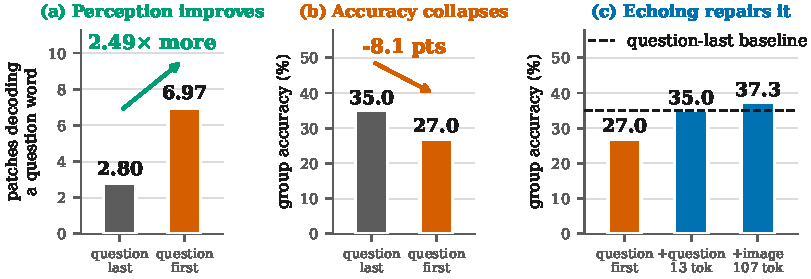
\includegraphics{figs/fig_teaser.pdf}
\end{center}
\caption{The question-first paradox and its repair, Qwen3-VL-8B.
\textbf{(a)} Question-first makes $2.49\times$ more image patches decode a
question content word (160 NaturalBench candidates), so the question reaches the
image. \textbf{(b)} It still loses $8.1$ points of group accuracy
($p = 1.3\times10^{-12}$). \textbf{(c)} Echoing the question after the image
repairs it for $13$ tokens; an $\tfrac{1}{8}$-resolution image echo beats the
baseline for $107$.}
\label{fig:teaser}
\end{figure}

Ask a vision-language model a question about an image and you must decide, often
without thinking about it, whether the question goes before the image or after
it. The information content is identical either way. Under causal attention,
putting the question first is the option that lets every image token see it,
which is what a reader would want when told to look for something specific.

It makes the model worse. Moving the question before the image costs Qwen3-VL-8B
$8.1$ points of NaturalBench group accuracy
($p = 1.3\times10^{-12}$), $9.5$ points on Winoground, and $18.0$ points on
CV-Bench, with an average loss of $7.0$ points across 13 benchmarks. The same
reversal holds for Qwen2.5-VL-7B, InternVL3-8B and LLaVA-1.5, which reaches
exactly zero group accuracy when the question comes first.

The obvious explanation is that question-first prompting damages perception, and
it is wrong. Reading image patches with a logit lens, question-first makes
$2.49\times$ more patches decode a content word from the question than
question-last does ($6.975$ against $2.800$ per image), and the question
measurably rewrites those tokens, moving them nearly twice as far from an
image-only forward pass as the system message alone. The ordering that looks most
like it has found the answer is the one that gets it wrong. We call this the
question-first paradox.

We locate the failure in read-out rather than perception. At the layer where the
answer position attends most strongly to the question, question-first sends
$2.19\times$ less attention mass there and $2.51\times$ more to the image. The
two orderings are indistinguishable at chance through layer 25 of 36 and then
diverge to $P(\text{correct})$ of $0.0986$ against $0.8747$. Severing attention
edges shows the dependence is causal and doubly dissociated: cutting the
answer-to-question path costs question-last $5.6$ points and question-first
nothing, while cutting the answer-to-image path costs question-first $9.6$ points
and question-last nothing.

That diagnosis prescribes the prompt. If the answer position cannot read the
question, put something after the image that it can read. Repeating the question
(\stit{}) costs $13$ tokens, recovers $78\%$ of the deficit, and provably cannot
change perception: the image tokens stay identical to five decimals. Repeating
the image (\sitit{}) recovers the deficit entirely and adds $1.18$ points over
question-last across 13 benchmarks. Neither repair supplies new information. A
reversed echo works as well as a correct one, and an eighth-resolution echo
matches a full one at $3\%$ of the added tokens. A reflective prompt optimizer,
given the same budget, gains only under the ordering the diagnosis says has
headroom and never reaches the question-last baseline it competes with.

\section{Related Work}
\label{sec:related}

\paragraph{Prompt order and position effects.} That the position of information
in a prompt changes what a model does is established in text. Few-shot example
order alone swings accuracy across a wide range \citep{fantasticallyordered2022},
and long-context models recover facts placed at the ends of a context better
than facts placed in the middle \citep{lostinthemiddle2024}, and both concern
where evidence sits relative to the query. The question-first
paradox is the multimodal counterpart with a sharper edge: our two layouts hold
the same tokens in the same quantity, so context length, truncation and
retrieval difficulty cannot distinguish them. Re-reading the question also helps
text reasoning \citep{rereading2024}, the same intervention as our question echo
reached from a different direction; that work motivates it as deliberation,
whereas our diagnosis says it restores an attention path.

\paragraph{Prompt optimization.} An alternative to reasoning about layout is to
search over prompt text. DSPy compiles declarative pipelines into tuned prompts
\citep{dspy2024}, and GEPA evolves prompts by reflecting on failures
\citep{gepa2025}. We use GEPA not as a competitor but as a test of the
diagnosis, because it can rewrite the system message and cannot move the image:
Section~\ref{sec:gepa} shows it recovers part of the loss under the broken
ordering and nothing under the working one, which is what a read-out account
predicts and a wording account does not.

\paragraph{Interpretability of vision-language models.} We read intermediate
states with a logit lens \citep{logitlens2020,tunedlens2023} and establish
causality by severing attention edges, the method used to localize factual
recall in language models \citep{attnknockout2023,rome2022}. Our use is
diagnostic rather than editing: we do not intervene to change behaviour at
deployment, only to identify which path an answer depends on. The
patch-difference procedure of Section~\ref{sec:anatomy-diff} adds a small piece
of method here, turning per-patch logit-lens decodes into an exhaustive,
rankable list of changes rather than a chosen illustration.

\paragraph{Relation to our own prior work.} This paper extends a workshop paper
by the present authors \citep{anon-workshop}, included in the supplementary
material for reviewers. We state the overlap plainly. That paper established the
question-first paradox on NaturalBench, POPE and Winoground, diagnosed it as a
read-out failure using the perception probe, the read-out probe and the
attention knockout, proposed question and image echoing as the repair, and
reported the reversed-echo control. Sections~\ref{sec:paradox}
and~\ref{sec:anatomy} recap that material in compressed form, with all numbers
reproduced on our own runs, because the new results are not interpretable
without it. Everything in Sections~\ref{sec:results} to~\ref{sec:ablations} is
new: fourteen further benchmarks including video and object detection, the
reversal of the effect under a detection objective, the echo-resolution sweep
and its exact token accounting, the automated patch-difference procedure, and
the prompt-optimizer comparison. The earlier paper named the second image's
token cost as an open limitation and did not measure it; measuring it, and
showing how little of the echo is needed, is the core of this one.

\section{The Question-First Paradox}
\label{sec:paradox}

This section and the next recap the phenomenon and diagnosis this paper extends
\citep{anon-workshop}, compressed to what the new results need. All numbers are
reproductions on our own runs.

\subsection{Notation and setup}
\label{sec:setup}

A prompt has three sections: the system message (S), the image (I), which
expands to many visual tokens, and the task or question (T). An ordering is
written as its sequence, so \sit{} is system-image-question and \sti{} is
system-question-image. An ordering may repeat a section: \stit{} repeats the
question after the image, \sitit{} repeats the image after the question, and
\sititrev{} is \sitit{} with the second image copy spatially reversed. The two
baselines are \sit{}, which is what most inference code emits by default, and
\sti{}, which is what a reader is told to do when looking for something
specific.

Qwen3-VL-8B \citep{qwen3vl} is the primary model and carries every analysis; for
breadth we also run Gemma-3-27B \citep{gemma3}, Gemma-4-31B \citep{gemma4},
Qwen2.5-VL-7B \citep{qwen25vl}, InternVL3-8B \citep{internvl3} and LLaVA-1.5
\citep{llava15}. All results use greedy decoding with a fixed answer-token
budget, and every ordering of a benchmark shares one system message, one question
string per item, one image preprocessing path and one scoring function, so
ordering is the only difference between columns.

Three benchmarks carry the diagnosis: NaturalBench \citep{naturalbench2024},
POPE \citep{pope2023} and Winoground \citep{winoground2022}.
Section~\ref{sec:results} adds fourteen not tested in prior work: RF20-VL,
twenty detection datasets drawn from RF100-VL \citep{rf100vl2025}, used both for
detection, scored by mAP, and as a $24{,}449$-question yes/no presence task over
the same images; nine image benchmarks (BLINK \citep{blink2024},
CV-Bench \citep{cambrian2024}, HR-Bench \citep{hrbench2025}, MMStar
\citep{mmstar2024}, MMVP \citep{mmvp2024}, RealWorldQA
\citep{realworldqa2024}, WorldMedQA-V \citep{worldmedqav2024}, TallyQA
\citep{tallyqa2019}, VQAv2 \citep{vqav2}); and four video QA benchmarks
(MVBench \citep{mvbench2024}, NExT-QA \citep{nextqa2021}, MSVD-QA
\citep{msvdqa2017}, TGIF-QA \citep{tgifqa2017}), where each \texttt{I} expands
to six uniformly sampled frames. Sizes are in the tables. For NaturalBench and
Winoground we pair on the group or example index and report an exact two-sided
McNemar test with a paired bootstrap 95\% interval over $5{,}000$ resamples.

\subsection{The phenomenon: moving the question earlier makes the model worse}
\label{sec:paradox-phenomenon}

Table~\ref{tab:ladder} runs six orderings on four benchmarks with Qwen3-VL-8B.
Every column uses the same system message, question string, image, decoding and
scoring code; \sti{} and \sit{} contain the same tokens in the same quantity.
Only the position of the question moves. Question-first is the worst ordering on
all four: NaturalBench group accuracy falls from $35.05$ to $26.95$
($p = 1.3\times10^{-12}$), Winoground from $31.75$ to $22.25$
($p = 7.7\times10^{-5}$), RF20 F1 from $78.57$ to $65.59$.

Intuition predicts the opposite. Placing the question first is what a reader
would do when told to look for something specific, and under causal attention it
is the only layout in which every image token can see the question.

\begin{table}[t]
\caption{Moving the question in front of the image is the worst choice on all
four benchmarks, and echoing it back is the best on three. Ordering ladder for
Qwen3-VL-8B, reproducing \citet{anon-workshop} and adding RF20. Bold marks the
best ordering in each row. POPE is the exception to the repair: plain
question-last already wins there. $N$ is 1{,}900 groups for NaturalBench,
9{,}000 items for POPE, 400 examples for Winoground and 24{,}449 for RF20.}
\label{tab:ladder}
\begin{center}
\small
\begin{tabular}{llrrrrrr}
\toprule
Benchmark & Metric & \ist{} & \sit{} & \sti{} & \stit{} & \sitit{} & \sititrev{} \\
\midrule
NaturalBench & pair acc.  & 78.93 & 79.21 & 75.29 & 78.95 & \best{80.36} & 80.26 \\
NaturalBench & group acc. & 33.95 & 35.05 & 26.95 & 35.00 & \best{37.37} & \best{37.37} \\
POPE         & F1         & 88.22 & \best{88.35} & 86.13 & 87.61 & 88.12 & 88.25 \\
Winoground   & group acc. & 28.00 & 31.75 & 22.25 & 37.50 & 40.25 & \best{41.00} \\
RF20         & F1         & 78.92 & 78.57 & 65.59 & 78.61 & \best{80.56} & 79.78 \\
\bottomrule
\end{tabular}
\end{center}
\end{table}

\section{Anatomy of the failure}
\label{sec:anatomy}

Two families of explanation come to mind for Section~\ref{sec:paradox}, and both
turn out to be wrong. The first is that question-first degrades the model's
perception of the image. The second is that it is a length or budget effect,
since the two layouts sit differently in the context window. We reject the
second immediately: \sti{} and \sit{} contain exactly the same tokens in a
different order, so their prompt lengths are identical to the token
(Table~\ref{tab:cost}). We spend the rest of this section rejecting the first,
and locating what actually breaks.

\subsection{The question does reach the image, and rewrites it}
\label{sec:anatomy-steering}

Putting the question before the image changes the image tokens themselves. We
compare each ordering's layer-18 image-token states against a run whose input is
the image alone, with no system message and no question, and take the mean
per-patch cosine. Under \ist{}, where nothing precedes the image, the patches are
the image-only patches (mean cosine $0.999998$ over $7{,}600$ pairs). Under
\sit{}, where only the system message precedes them, it falls to $0.9110$. Under
\sti{} it falls to $0.8627$, with the most affected patch at $0.6149$, so the
question-specific rewrite is about $1.8\times$ the size of the system message's
own effect.

Causal masking gives a free control here, and it also explains a later result.
Echoing the question \emph{after} the image (\stit{}) cannot alter the image
tokens, and the measurement confirms it to five decimals:
$\cos(\sti{}, \stit{}) = 0.99999$. Whatever \stit{} does for accuracy, it does
without touching perception.

\subsection{What breaks is read-out, and it breaks late}
\label{sec:anatomy-readout}

If perception is intact, the failure has to be downstream of it. We probe the
answer position directly on the $150$ NaturalBench pairs where \sti{} is wrong
and \sit{} is right, tracking how much attention mass the answer position sends
to the question span and to the image span at each of the model's 36 layers.

At layer 23, where answer-to-question attention peaks for both orderings, \sti{}
sends $0.0676$ of its mass to the question while \sit{} sends $0.1479$, a
$2.19\times$ deficit. Attention to the image runs the other way, peaking at
$0.2367$ for \sti{} against $0.0942$ for \sit{}. Averaged over layers 20 to 35,
the ratio of question to image attention is $0.424$ under \sti{} and $1.065$
under \sit{}. Question-first leaves the answer position staring at the image it
has already encoded, and not at the question it is supposed to answer.

The timing matters as much as the size. Tracking $P(\text{correct})$ over the
$\{$Yes, No$\}$ decision at each layer on $300$ pairs, the two orderings are
indistinguishable at chance ($\approx 0.50$) through layer 25. They separate at
layer 26 and never re-cross: by layer 34, \sti{} is at $0.0986$ and \sit{} at
$0.8747$. A failure that only appears in the last quarter of the network is not
an encoding failure. Logit-lens $P(\text{gt})$ at the final layer tells the same
story, $0.1346$ for \sti{} against $0.8485$ for \sit{}.

\begin{figure}[t]
\begin{center}
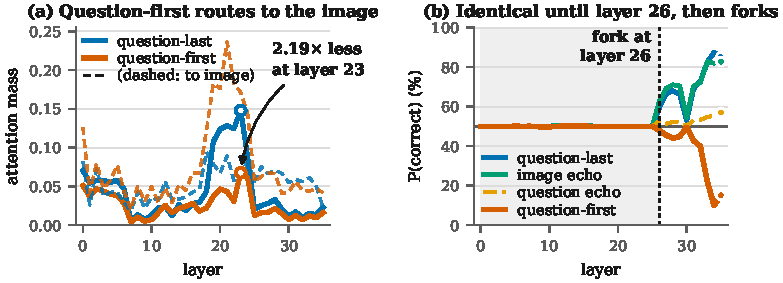
\includegraphics{figs/fig_mechanism.pdf}
\end{center}
\caption{Where question-first breaks (150 NaturalBench pairs where it is wrong
and question-last is right). \textbf{(a)} Attention leaving the answer position,
to the question (solid) and the image (dashed): at layer 23 question-first sends
$2.19\times$ less to the question. \textbf{(b)} $P(\text{correct})$ per layer.
The two baselines sit at chance through layer 25, fork at 26 and never re-cross;
both echo orderings track question-last.}
\label{fig:mechanism}
\end{figure}

\begin{finding}
\textbf{Finding.} The failure is read-out, not perception, and it is late.
Question-first sends $2.19\times$ less attention from the answer position to the
question at the peak read-out layer ($0.0676$ vs $0.1479$), the two orderings
are indistinguishable until layer 26 of 36, and they then diverge to
$P(\text{correct})$ of $0.0986$ versus $0.8747$.
\end{finding}

\subsection{A causal test: severing the two paths dissociates the orderings}
\label{sec:anatomy-knockout}

\begin{wrapfigure}{r}{0.44\textwidth}
\vspace{-14pt}
\begin{center}
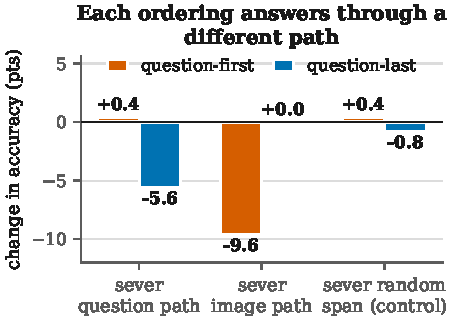
\includegraphics[width=0.42\textwidth]{figs/fig_knockout.pdf}
\end{center}
\vspace{-9pt}
\caption{Attention knockout, 250 NaturalBench pairs, query side restricted to
the answer position. Bars are change against the unmodified run.}
\label{fig:knockout}
\vspace{-10pt}
\end{wrapfigure}
The attention numbers are correlational. To show that the question path is what
\sit{} depends on and the image path is what \sti{} depends on, we sever each
one and measure the damage. We zero the attention edges from the answer position
to the question span (\texttt{ko\_question}) or to the image span
(\texttt{ko\_image}), on $250$ NaturalBench pairs, and add a control that severs
an equal-length random span of pre-image text (\texttt{ko\_random}) so that any
effect of merely removing attention mass is accounted for.

The result is a clean double dissociation (Figure~\ref{fig:knockout}). Cutting
the answer-to-question path costs \sit{} $5.6$ points ($58.8 \to 53.2$, paired
bootstrap 95\% CI $[+1.99, +9.60]$) and costs \sti{} nothing at all ($+0.4$).
Cutting the answer-to-image path costs \sti{} $9.6$ points ($57.6 \to 48.0$) and
costs \sit{} exactly zero. The random-span control moves both orderings by at
most $0.8$ points, so neither effect is an artifact of removing attention mass.

Question-last answers by reading the question. Question-first answers by reading
the image, having already folded its reading of the question into those image
tokens, and that is the path that does not carry the answer.


\begin{finding}
\textbf{Finding.} The two orderings answer through different paths, and we show
it causally. Severing answer-to-question costs \sit{} $5.6$ points (95\% CI
$[+1.99, +9.60]$) and \sti{} nothing ($+0.4$); severing answer-to-image costs
\sti{} $9.6$ points and \sit{} nothing ($0.0$); a span-size control moves both
by $\leq 0.8$.
\end{finding}

\section{From Diagnosis to Prompt: Echoing}
\label{sec:echoing}

The diagnosis prescribes the prompt with no design freedom left. If the answer
position cannot read the question, put something after the image that it can
read. There are exactly two things available.

\paragraph{Question echoing (\stit{}).} Repeat the question after the image.
This restores question-answer adjacency while provably leaving perception
untouched, since causal masking means a later copy cannot alter earlier patches
($\cos(\sti{}, \stit{}) = 0.99999$, Section~\ref{sec:anatomy-steering}). It
costs $13$ tokens, and it is the controlled intervention the diagnosis calls
for: matched on content, matched on perception, differing only in whether the
answer position has a question to read.

\paragraph{Image echoing (\sitit{}).} Repeat the image after the question, so
the answer position has both a nearby question and image tokens encoded with the
question already in context. Prior work also reversed the echoed copy
(\sititrev{}) and found it changed little, which we reproduce: NaturalBench
group accuracy moves from $37.37$ to $37.37$ ($p = 1.00$) and Winoground from
$40.25$ to $41.00$ ($p = 0.68$).

Two results in Table~\ref{tab:ladder} keep us honest. Question echoing alone is
not reliably better than simply asking the question last (NaturalBench $35.00$
against $35.05$, $p = 1.00$), so its role is to repair question-first prompting,
not to improve on question-last. Image echoing is a real gain and is the claim
we defend ($+0.085$ on Winoground, $p = 2.4\times10^{-5}$), though on POPE it
does not help at all.

What prior work left open is what the echo is made of and what it costs. It
listed the second image's token cost as a limitation and did not measure it.
Sections~\ref{sec:results} and~\ref{sec:ablations} take up that thread: how far
the paradox reaches, where the repair stops working, how little of the echo is
needed, and whether a prompt optimizer would have found it anyway.

\section{Generality and boundaries}
\label{sec:generality}

Prior work tested three yes/no benchmarks. That leaves open whether the paradox
is a property of yes/no visual question answering, of those three datasets, or
of the prompt layout itself. We run the full ordering ladder on 13 further
benchmarks spanning single-image perception, high-resolution perception,
counting, medical VQA and four video QA datasets, and separately on RF20, a
$24{,}449$-item presence-detection benchmark built from 20 detection datasets
across 7 categories.

\subsection{The paradox holds on 13 new benchmarks}

Moving the question from after the image to before it costs Qwen3-VL-8B $7.01$
points on average and hurts on 12 of 13 (Table~\ref{tab:breadth}). The effect is
far larger than the differences that usually separate published models:
CV-Bench loses $18.01$ points, MMStar $11.40$, MMVP $9.00$, NExT-QA $8.91$.
WorldMedQA-V is the single benchmark where question-first is not worse
($+1.06$); we report it rather than dropping it, and note it is also the
smallest benchmark in the set ($N = 568$).

The two echo orderings separate the cost of the repair from its size. Question
echoing recovers $5.49$ of the $7.01$ points, or $78\%$ of the deficit, for $13$
extra tokens. Image echoing recovers all of it and exceeds question-last by
$1.18$ points, winning on 9 of 13.

\begin{table}[t]
\caption{Full ordering ladder for Qwen3-VL-8B across 13 benchmarks not tested in
prior work, video QA below the rule. Best of the four orderings in bold. The
echo column gives \sitit{} with the second image copy at half resolution.
Question-first hurts on 12 of 13; image echoing recovers the loss on the image
benchmarks and does not on video.}
\label{tab:breadth}
\begin{center}
\small
\begin{tabular}{lrrrrrrrr}
\toprule
 & & \multicolumn{4}{c}{Ordering} & Echo $\tfrac{1}{2}$ & \multicolumn{2}{c}{$\Delta$ vs \sit{}} \\
\cmidrule(lr){3-6}\cmidrule(lr){8-9}
Benchmark & $N$ & \sit{} & \sti{} & \stit{} & \sitit{} & \sitit{} & \sti{} & \sitit{} \\
\midrule
BLINK         &         793 & 53.09 & 44.51 & 52.21 & \best{53.97} & 50.44 & $-8.58$ & $+0.88$ \\
CV-Bench      &     2{,}638 & 81.35 & 63.34 & 79.98 & \best{83.55} & 83.70 & $-18.01$ & $+2.20$ \\
HR-Bench      &     1{,}600 & 67.81 & 59.25 & 63.94 & \best{69.75} & 68.44 & $-8.56$ & $+1.94$ \\
MMStar        &     1{,}500 & 53.33 & 41.93 & 51.47 & \best{55.13} & 56.07 & $-11.40$ & $+1.80$ \\
MMVP          &         300 & 73.00 & 64.00 & 72.33 & \best{77.67} & 76.00 & $-9.00$ & $+4.67$ \\
RealWorldQA   &         765 & 69.28 & 63.92 & 67.19 & \best{70.33} & 70.33 & $-5.36$ & $+1.05$ \\
WorldMedQA-V  &         568 & 53.35 & 54.40 & 56.87 & \best{57.22} & 57.57 & $+1.06$ & $+3.87$ \\
TallyQA       &    38{,}589 & 79.14 & 74.15 & 77.85 & \best{79.99} & 79.36 & $-5.00$ & $+0.84$ \\
VQAv2         &   214{,}354 & \best{81.66} & 78.72 & 80.49 & 81.30 & 81.38 & $-2.94$ & $-0.36$ \\
\cmidrule(lr){1-9}
\multicolumn{2}{l}{\emph{Mean, 9 image}} & & & & & & $-7.53$ & $+1.88$ \\
\midrule
MVBench       &     2{,}600 & 64.08 & 55.88 & 62.23 & \best{64.62} & 66.08 & $-8.19$ & $+0.54$ \\
NExT-QA       &     8{,}564 & \best{78.21} & 69.30 & 76.05 & 77.95 & 78.11 & $-8.91$ & $-0.26$ \\
MSVD-QA       &    13{,}157 & \best{40.05} & 35.52 & 36.61 & 39.27 & 39.51 & $-4.53$ & $-0.78$ \\
TGIF-QA       &    25{,}751 & \best{36.32} & 34.59 & 33.62 & 35.26 & 35.50 & $-1.74$ & $-1.06$ \\
\cmidrule(lr){1-9}
\multicolumn{2}{l}{\emph{Mean, 4 video}} & & & & & & $-5.84$ & $-0.39$ \\
\bottomrule
\end{tabular}
\end{center}
\end{table}

\begin{finding}
\textbf{Finding.} The paradox is a property of the layout, not of yes/no visual
question answering. Across 13 benchmarks never previously tested, question-first
costs $7.01$ points on average and hurts on 12 of 13, with a worst case of
$18.01$ points on CV-Bench, while prompt content is held identical.
\end{finding}

\subsection{RF20: a category where question-first more than halves accuracy}
\label{sec:generality-rf20}

RF20 asks whether a given object class is present in a detection-style image,
over $24{,}449$ items drawn from 20 datasets in 7 categories. It is the hardest
test of generality here because its images are not web photographs and its
questions are not natural language questions about scenes.

Question-first hurts on all 7 categories, by $11.36$ points on average
(Table~\ref{tab:rf20}). On Lab Imaging it does not merely hurt: accuracy falls
from $86.29$ to $38.94$, a loss of $47.35$ points, which is below the rate this
binary task would get by answering a single class blindly. Industrial loses
$14.26$. Both are domains where the target is a small, low-contrast region and
the decision hinges on evidence the model must go back and look at, which is
exactly the read-out the question-first layout strands.

Echoing repairs the collapse and then some. On Lab Imaging, question echoing
reaches $91.71$ and image echoing $90.93$, against question-last's $86.29$,
so the ordering that broke the category worst is also the one the cheaper repair
helps most.

\begin{table}[t]
\caption{RF20 accuracy by category, Qwen3-VL-8B, $24{,}449$ items. Question-first
hurts on 7 of 7 categories. Lab Imaging loses $47.35$ points, and both echo
orderings recover it past the question-last baseline.}
\label{tab:rf20}
\begin{center}
\small
\begin{tabular}{lrrrrrrr}
\toprule
Category & $N$ & \sit{} & \sti{} & \stit{} & \sitit{} & $\Delta$ \sti{} & $\Delta$ \sitit{} \\
\midrule
Document    & 10{,}200 & 80.94 & 76.20 & 80.30 & \best{84.19} & $-4.74$ & $+3.25$ \\
Misc        &  4{,}114 & 85.71 & 82.50 & \best{85.90} & 85.05 & $-3.21$ & $-0.66$ \\
Industrial  &  2{,}958 & \best{82.45} & 68.19 & 81.54 & 82.18 & $-14.26$ & $-0.27$ \\
Lab Imaging &  2{,}822 & 86.29 & 38.94 & \best{91.71} & 90.93 & $-47.35$ & $+4.64$ \\
Sport       &  2{,}654 & 49.06 & 48.61 & 42.99 & \best{51.96} & $-0.45$ & $+2.90$ \\
Flora/Fauna &  1{,}592 & 86.56 & 82.54 & \best{87.44} & 86.75 & $-4.02$ & $+0.19$ \\
Aerial      &      109 & \best{94.50} & 88.99 & 89.91 & \best{94.50} & $-5.51$ & $+0.00$ \\
\midrule
\multicolumn{2}{l}{\emph{Mean over 7}} & & & & & $-11.36$ & $+1.44$ \\
\bottomrule
\end{tabular}
\end{center}
\end{table}

\begin{finding}
\textbf{Finding.} Question-first can be catastrophic, not merely costly. On
RF20's Lab Imaging category it takes accuracy from $86.29$ to $38.94$, a
$47.35$-point loss, and it hurts on 7 of 7 categories. Echoing recovers the
category to $91.71$, above the question-last baseline.
\end{finding}

\subsection{Where the repair stops: video}
\label{sec:generality-video}

The four video QA datasets draw a boundary the original benchmarks could not.
The paradox itself is if anything more reliable there: question-first hurts on 4
of 4, by $5.84$ points on average. The repair, however, splits by which thing is
echoed. Question echoing still recovers $3.31$ of those points. Image echoing
does not: it beats question-last on only 1 of 4 video datasets and loses $0.39$
points on average, against $+1.88$ on the nine image benchmarks.

The reason is mechanical rather than mysterious. For video the ``image'' is a
frame sequence, so an image echo doubles a visual context that is already long,
and the read-out surface it adds is buried behind far more tokens than in the
single-image case. The practical rule is to echo the question on video and the
image on stills.

\begin{finding}
\textbf{Finding.} The paradox and its repair have different domains. On video,
question-first still hurts on 4 of 4 datasets ($-5.84$), but image echoing helps
on only 1 of 4 ($-0.39$ on average, against $+1.88$ on nine image benchmarks),
while question echoing still recovers $+3.31$. Echo the question on video, the
image on stills.
\end{finding}

\section{Ablations: what the echo is actually made of}
\label{sec:ablations}

The diagnosis in Section~\ref{sec:background} makes a strong claim about what the
second image copy is for. It is not there to be re-perceived. It is there to put
image tokens after the question so the read-out step has something local to
attend to. That claim has a sharp consequence: the echoed copy should not need to
be legible. We test it by degrading the echo, by pricing it, and by asking
whether a prompt optimizer that can only edit text finds the same fix.

\subsection{The echoed copy does not need to be legible}
\label{sec:ablation-resolution}

We downscale only the second image occurrence in \sitit{}, leaving the first at
full resolution, and sweep the echo scale over $1$, $\tfrac{1}{2}$,
$\tfrac{1}{4}$ and $\tfrac{1}{8}$ (Table~\ref{tab:resolution}). On three of four
benchmarks a quarter-resolution echo matches or beats a full-resolution one:
POPE moves by $-0.05$ F1, Winoground by $+0.75$ group accuracy, and NaturalBench
by $+0.21$ pair accuracy.

Pushing to an eighth makes the point sharper. On NaturalBench, an echo carrying
$\tfrac{1}{64}$ of the original pixels scores $37.32$ group accuracy against the
full echo's $37.37$, a difference of $0.001$ with $p = 1.00$, while still beating
question-last by $+0.023$ ($p = 0.005$). The echo can be destroyed as an image
and keep its entire benefit.

RF20 is the exception, and it is the informative one. Its accuracy falls
monotonically as the echo degrades ($-0.50$ F1 at half, $-1.76$ at quarter).
RF20 asks whether a specific, often small object class is present in a
detection-style image, so the second look is doing real perceptual work there
rather than only re-anchoring. The split between RF20 and the other three says
the echo has two separable jobs, and that only one of them needs pixels.

\begin{figure}[t]
\begin{minipage}[t]{0.50\textwidth}
\vspace{0pt}
\centering
\captionof{table}{Echo-resolution sweep, Qwen3-VL-8B. Only the \emph{second}
image occurrence is downscaled; the first stays at full resolution. Three of four
benchmarks are flat or better at quarter resolution. RF20, whose targets are
small, degrades monotonically. Metrics are F1 for POPE and the RF20 presence task, group accuracy for Winoground, pair accuracy for NaturalBench. Blank cells were not run.}
\label{tab:resolution}
\vspace{2pt}
\small
\setlength{\tabcolsep}{3.5pt}
\begin{tabular}{lrrrr}
\toprule
Benchmark & Echo $1$ & $\tfrac{1}{2}$ & $\tfrac{1}{4}$ & $\tfrac{1}{8}$ \\
\midrule
POPE         & 88.12 & \best{88.35} & 88.07 & \\
Winoground   & 40.25 & \best{41.75} & 41.00 & \best{41.75} \\
NaturalBench & 80.36 & 80.55 & \best{80.57} & 80.18 \\
RF20 (presence) & \best{80.56} & 80.06 & 78.80 & \\
\bottomrule
\end{tabular}
\end{minipage}\hfill
\begin{minipage}[t]{0.47\textwidth}
\vspace{0pt}
\centering
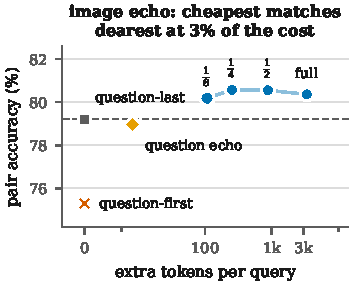
\includegraphics[width=\linewidth]{figs/fig_pareto.pdf}
\caption{Cost against accuracy on NaturalBench. The $x$ axis is extra tokens per
query versus question-first (symmetric log, so $0$ is shown); the dashed line is
question-last. Every image echo clears that baseline, and the
$\tfrac{1}{8}$-resolution echo ($+107$ tokens) is indistinguishable from the full
one ($+3{,}352$).}
\label{fig:pareto}
\end{minipage}
\end{figure}

\begin{finding}
\textbf{Finding.} The echoed image does not need to be legible. An
eighth-resolution echo, carrying $\tfrac{1}{64}$ of the pixels, is statistically
indistinguishable from a full-resolution one on NaturalBench ($37.32$ vs
$37.37$ group accuracy, $p = 1.00$) while still beating question-last
($p = 0.005$). Only RF20, whose targets are small, needs the pixels
($-1.76$ F1 at quarter resolution).
\end{finding}

\subsection{What echoing costs}
\label{sec:ablation-cost}

Prompt-level interventions are usually reported without their bill. We count
exact token counts for each ordering with the Qwen3-VL-8B processor over 20
images spanning RF20's constituent datasets, separating vision from text tokens
(Table~\ref{tab:cost} in Appendix~\ref{app:cost}).

The two echo mechanisms are three orders of magnitude apart. Repeating the
question costs $13$ tokens. Repeating the image at full resolution costs
$3{,}352$, which roughly doubles the prompt. Downscaling the echo collapses that
cost quickly, because vision-token count falls with area: a half-resolution echo
costs $875$ added tokens, a quarter-resolution echo $252$, and an
eighth-resolution echo $107$. Figure~\ref{fig:pareto} puts the two axes
together. The accuracy curve is flat across a $31\times$ range of echo cost, so
the operating point to ship is the cheapest one.


\begin{finding}
\textbf{Finding.} Echo cost is a tunable knob, not a fixed doubling of the
prompt. A full-resolution image echo adds $3{,}352$ tokens per query, but a
quarter-resolution echo adds $252$ ($7.5\%$) and an eighth-resolution echo adds
$107$ ($3.2\%$) for indistinguishable accuracy, while question echoing adds $13$.
\end{finding}

\subsection{Prompt optimization finds part of the fix, and only where the
mechanism says it should}
\label{sec:ablation-gepa}
\label{sec:gepa}

A reviewer will reasonably ask whether careful prompt engineering would do the
same work as echoing, making the ordering story incidental. We test this with
GEPA \citep{gepa2025}, a reflective prompt optimizer, and use it as a prediction
test rather than as a baseline to beat.

The mechanism predicts an asymmetry. GEPA may rewrite the system message text
but cannot move the image, so it cannot repair a read-out failure caused by
token order. It should find recoverable headroom under \sti{}, where read-out is
broken, and little or nothing under \sit{}, where it is not. That is what
happens (Table~\ref{tab:gepa}, Appendix~\ref{app:gepa}). Under \sti{}, GEPA
improves all three benchmarks: POPE $86.41 \to 87.25$, VQAv2 $86.11 \to 88.13$,
NaturalBench $74.74 \to 75.79$. Under \sit{}, the same optimizer with the same
budget returns the seed prompt unchanged on POPE and VQAv2, both exact ties, and
regresses NaturalBench by $0.41$ by overfitting its validation split.

Two further numbers matter. First, \sit{}'s baseline is higher than \sti{}'s on
every benchmark ($88.27$ vs $86.41$, $88.55$ vs $86.11$, $78.80$ vs $74.74$),
so the asymmetry is a headroom effect and not a quirk of the optimizer. Second,
GEPA's best \sti{} prompt never reaches the plain \sit{} baseline: it closes
$26\%$ to $83\%$ of the \sti{}-to-\sit{} gap and stops there. Its optimized
prompts add $26$, $32$ and $71$ tokens per query, less than even an
eighth-resolution echo, but its search costs $157{,}725$ to $982{,}343$ tokens
once plus a separate reflection model. Rewording the prompt recovers part of
what bad ordering costs. Moving or echoing the image recovers the rest.

\begin{table}[t]
\caption{GEPA prompt optimization under two orderings, Qwen3-VL-8B, on held-out
evaluation sets. GEPA finds real gains under \sti{} and nothing under \sit{},
as the read-out diagnosis predicts. It never reaches the \sit{} baseline it is
competing with.}
\label{tab:gepa}
\begin{center}
\small
\setlength{\tabcolsep}{4pt}
\begin{tabular}{llrrrrr}
\toprule
 & & & \multicolumn{2}{c}{Accuracy} & & Gap \\
\cmidrule(lr){4-5}
Benchmark & Order & $N$ & Seed & GEPA & $\Delta$ & closed \\
\midrule
\multirow{2}{*}{POPE}         & \sti{} & 8{,}800 & 86.41 & 87.25 & $+0.84$ & $45\%$ \\
                              & \sit{} & 8{,}800 & 88.27 & 88.27 & $+0.00$ & n/a \\
\midrule
\multirow{2}{*}{VQAv2}        & \sti{} & 10{,}000 & 86.11 & 88.13 & $+2.02$ & $83\%$ \\
                              & \sit{} & 10{,}000 & 88.55 & 88.55 & $+0.00$ & n/a \\
\midrule
\multirow{2}{*}{NaturalBench} & \sti{} & 7{,}000 & 74.74 & 75.79 & $+1.04$ & $26\%$ \\
                              & \sit{} & 7{,}000 & 78.80 & 78.39 & $-0.41$ & n/a \\
\bottomrule
\end{tabular}
\end{center}
\end{table}

\begin{finding}
\textbf{Finding.} Prompt optimization behaves exactly as the read-out diagnosis
predicts: GEPA gains under \sti{} (POPE $+0.84$, VQAv2 $+2.02$, NaturalBench
$+1.04$) and finds nothing under \sit{} (two exact ties and $-0.41$), because
\sit{} has less headroom to recover. It closes $26\%$ to $83\%$ of the
\sti{}-to-\sit{} gap and never reaches the \sit{} baseline, so rewording is not
a substitute for fixing token order.
\end{finding}

\section{Discussion}
\label{sec:discussion}

The standard picture of a vision-language model answering a question is that the
question selects what to look for and the model then looks. Under question-first
prompting the first half of that picture is measurably correct: the question
reaches the image and rewrites its tokens, and $2.49\times$ more patches decode
the question's own words. The model still answers worse. The missing step is that
the evidence has to be read back out at the answer position, through attention
paths that token order determines. This is why the fix is so cheap relative to
its size: nothing has to be learned and nothing has to be re-perceived. The
intervention is not supplying information, it is putting a read-out surface where
the answer position can reach it.

\paragraph{Implications beyond prompt ordering.} For benchmarking, an unreported
prompt-layout choice is a confound of the same size as the model differences
benchmarks are built to detect: question-first versus question-last moves
CV-Bench by $18.01$ points, so two implementations of ``the same'' prompt can
differ by more than the gap being measured. For deployed and agentic systems,
pipelines that prepend a goal to a growing context and then append retrieved
images produce question-first layouts by construction and pay for it silently;
appending a one-line restatement of the request after the visual content costs
$13$ tokens. For training recipes, the failure lives in the read-out path rather
than in perception, which suggests instruction tuning that varies section order
rather than fixing one canonical template, and the Gemma models show the failure
is trainable away.

\paragraph{Limitations.} The diagnosis is established on Qwen3-VL-8B. The paradox
replicates on Qwen2.5-VL-7B, InternVL3-8B and LLaVA-1.5 but not on either Gemma
model, so the read-out account describes a common failure mode rather than a
property of the architecture; image echoing still helps the Gemma models, but the
mechanism we document cannot be the reason there. Image echoing is also not
uniformly right: it does not beat question-last on POPE ($88.12$ against $88.35$
F1), and on the four video QA benchmarks it loses to question-last on three of
four. Finally, our knockout result depends on restricting the query side to the
answer position; widening it does not reproduce the question-side half of the
dissociation, and the span-size control is itself large there, so we treat the
broader scope as uninformative rather than as contrary evidence
(Appendix~\ref{app:repro}).

\section*{Reproducibility, AI Use, and Ethics Statements}
\textbf{Reproducibility.}
Models, benchmarks and protocol: Section~\ref{sec:setup}. Per-run detail,
including the two configuration choices that change a result if missed:
Appendices~\ref{app:rf20presence}--\ref{app:repro}. Every accuracy is read from
a per-run result file, and significance tests use paired McNemar with a paired
bootstrap over $5{,}000$ resamples at a fixed seed. Code and the figure scripts,
which regenerate every figure from those result files, are provided in the
supplementary material together with the prior workshop paper this work extends,
and will be released publicly.
%
\textbf{AI use.}
AI tools helped with code and editing; the authors reviewed all of it and take
full responsibility.
%
\textbf{Ethics.}
We audit existing, publicly released models on public research benchmarks,
collecting no new data and involving no human subjects. RF20 includes
surveillance-adjacent detection domains, so the usual dual-use risk of detection
systems applies. Our intervention improves accuracy without fine-tuning but does
nothing about the biases these models already carry; a more accurate answer is
not a fairer one. We report where it fails, on video and POPE, so that it is not
applied where it does not help.


\bibliography{main}
\bibliographystyle{iclr2027_conference}

\newpage
\appendix
\begin{center}
  {\LARGE\bfseries Appendix}
\end{center}
\section{RF20 presence task: the yes/no variant}
\label{app:rf20presence}

Besides the detection task of Section~\ref{sec:generality-rf20}, RF20's images
support a yes/no presence question ("is a \textless class\textgreater\ in the
image?"), $24{,}449$ questions over 20 datasets in 7 categories. This variant
has the same answer format as NaturalBench, POPE and Winoground, and it behaves
like them: question-first hurts on 7 of 7 categories, by $11.36$ points on
average. On Lab Imaging it takes accuracy from $86.29$ to $38.94$, a $47.35$
point loss, and both echo orderings recover the category past the question-last
baseline. The contrast with Table~\ref{tab:rf20map}, where the same images under
a detection objective show the opposite sign, is the cleanest evidence we have
that the paradox tracks the answer format rather than the imagery.

\begin{table}[h]
\caption{RF20 presence task, accuracy by category, Qwen3-VL-8B, $24{,}449$
questions. Question-first hurts on 7 of 7 categories, opposite in sign to the
detection results on the same images.}
\label{tab:rf20}
\begin{center}
\small
\begin{tabular}{lrrrrrrr}
\toprule
Category & $N$ & \sit{} & \sti{} & \stit{} & \sitit{} & $\Delta$ \sti{} & $\Delta$ \sitit{} \\
\midrule
Document    & 10{,}200 & 80.94 & 76.20 & 80.30 & \best{84.19} & $-4.74$ & $+3.25$ \\
Misc        &  4{,}114 & 85.71 & 82.50 & \best{85.90} & 85.05 & $-3.21$ & $-0.66$ \\
Industrial  &  2{,}958 & \best{82.45} & 68.19 & 81.54 & 82.18 & $-14.26$ & $-0.27$ \\
Lab Imaging &  2{,}822 & 86.29 & 38.94 & \best{91.71} & 90.93 & $-47.35$ & $+4.64$ \\
Sport       &  2{,}654 & 49.06 & 48.61 & 42.99 & \best{51.96} & $-0.45$ & $+2.90$ \\
Flora/Fauna &  1{,}592 & 86.56 & 82.54 & \best{87.44} & 86.75 & $-4.02$ & $+0.19$ \\
Aerial      &      109 & \best{94.50} & 88.99 & 89.91 & \best{94.50} & $-5.51$ & $+0.00$ \\
\midrule
\multicolumn{2}{l}{\emph{Mean over 7}} & & & & & $-11.36$ & $+1.44$ \\
\bottomrule
\end{tabular}
\end{center}
\end{table}

\section{Attention knockout in full}
\label{app:knockout}

Qwen3-VL-8B, 250 NaturalBench pairs, query side restricted to the answer
position. \texttt{ko\_question} severs the attention edges from the answer
position to the question span, \texttt{ko\_image} to the image span, and
\texttt{ko\_random} to an equal-length random span of pre-image text as a
span-size control.

\begin{figure}[h]
\begin{center}
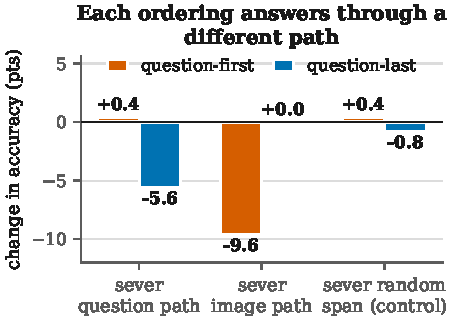
\includegraphics[width=0.52\textwidth]{figs/fig_knockout.pdf}
\end{center}
\caption{Each ordering answers through a different path. Bars are the change in
accuracy against the unmodified run ($57.6$ for question-first, $58.8$ for
question-last). Severing answer-to-question hurts only question-last; severing
answer-to-image hurts only question-first; the random span-size control moves
both by at most $0.8$ points.}
\label{fig:knockout}
\end{figure}

The paired bootstrap on the question-last question knockout gives
$\Delta = 0.056$ with a 95\% CI of $[+0.0199, +0.096]$, so the interval excludes
zero.

\section{Cross-model ladders in full}
\label{app:models}

\begin{table}[h]
\caption{NaturalBench ladder across five models ($1{,}900$ groups). Four of five
models lose accuracy when the question moves before the image. Missing entries
were not run. LLaVA-1.5's question-first group accuracy is exactly zero.}
\label{tab:models-nb}
\begin{center}
\small
\begin{tabular}{llrrrrr}
\toprule
Model & Metric & \sit{} & \sti{} & \stit{} & \sitit{} & $\Delta$ (\sti{}$-$\sit{}) \\
\midrule
Qwen3-VL-8B   & pair acc.  & 79.21 & 75.29 & 78.95 & \best{80.36} & $-3.92$ \\
              & group acc. & 35.05 & 26.95 & 35.00 & \best{37.37} & $-8.10$ \\
Qwen2.5-VL-7B & pair acc.  & \best{76.05} & 64.95 & 71.83 & 75.71 & $-11.10$ \\
              & group acc. & \best{27.74} & 10.16 & 19.11 & 27.63 & $-17.58$ \\
InternVL3-8B  & pair acc.  & 79.63 & 75.61 & 79.76 & \best{80.80} & $-4.02$ \\
              & group acc. & 35.53 & 27.63 & 36.47 & \best{39.32} & $-7.90$ \\
LLaVA-1.5     & pair acc.  & \best{66.87} & 50.26 & 66.29 & n/a & $-16.61$ \\
              & group acc. & \best{12.32} & 0.00 & 12.05 & n/a & $-12.32$ \\
Gemma-3-27B   & pair acc.  & 73.34 & 73.21 & \best{74.64} & 74.61 & $-0.13$ \\
              & group acc. & 22.63 & 23.21 & 25.26 & \best{25.53} & $+0.58$ \\
\bottomrule
\end{tabular}
\end{center}
\end{table}

\begin{table}[h]
\caption{Cross-model check on the four benchmarks run for all three models. The
question-first paradox does not replicate on either Gemma model, yet image
echoing is still the best ordering on 7 of 8 model-benchmark pairs.}
\label{tab:crossmodel}
\begin{center}
\small
\begin{tabular}{llrrrrrrr}
\toprule
 & & & \multicolumn{4}{c}{Ordering} & \multicolumn{2}{c}{$\Delta$ vs \sit{}} \\
\cmidrule(lr){4-7}\cmidrule(lr){8-9}
Model & Benchmark & $N$ & \sit{} & \sti{} & \stit{} & \sitit{} & \sti{} & \sitit{} \\
\midrule
\multirow{4}{*}{Gemma-3-27B}
 & BLINK   &     793 & 44.51 & 43.51 & 42.75 & \best{44.89} & $-1.01$ & $+0.38$ \\
 & MMVP    &     300 & 72.67 & 72.33 & 72.00 & \best{74.67} & $-0.33$ & $+2.00$ \\
 & TallyQA &  38{,}589 & 63.00 & 67.60 & 68.93 & \best{69.97} & $+4.60$ & $+6.96$ \\
 & VQAv2   & 214{,}354 & \best{64.77} & 62.07 & 63.04 & 62.07 & $-2.70$ & $-2.70$ \\
\cmidrule(lr){2-9}
 & \emph{Mean} & & & & & & $+0.14$ & $+1.66$ \\
\midrule
\multirow{4}{*}{Gemma-4-31B}
 & BLINK   &     793 & 54.48 & 56.12 & 56.12 & \best{56.49} & $+1.64$ & $+2.02$ \\
 & MMVP    &     300 & 84.67 & 86.00 & 86.67 & \best{87.33} & $+1.33$ & $+2.67$ \\
 & TallyQA &   2{,}000 & 80.65 & 80.50 & 81.20 & \best{82.60} & $-0.15$ & $+1.95$ \\
 & VQAv2   &   3{,}000 & 73.50 & 74.66 & 75.65 & \best{76.00} & $+1.16$ & $+2.50$ \\
\cmidrule(lr){2-9}
 & \emph{Mean} & & & & & & $+1.00$ & $+2.28$ \\
\bottomrule
\end{tabular}
\end{center}
\end{table}

\section{Significance tests in full}
\label{app:significance}

Paired on group index (NaturalBench) or example index (Winoground), exact
two-sided McNemar plus a paired bootstrap 95\% CI over $5{,}000$ resamples,
seed 0. Accuracies are group accuracy.

\begin{table}[h]
\caption{Significance for consecutive rungs of the ladder and for the headline
comparisons. \sti{} versus \sit{} is highly significant for Qwen3-VL-8B on both
benchmarks and absent for Gemma-3-27B. \sitit{} versus \sit{} is significant on
Winoground for both models.}
\label{tab:significance}
\begin{center}
\scriptsize
\setlength{\tabcolsep}{3pt}
\begin{tabular}{lllrrrl}
\toprule
Benchmark & Model & Comparison & acc A & acc B & $\Delta$ (95\% CI) & McNemar $p$ \\
\midrule
NaturalBench & Qwen3-VL-8B & \sti{} vs \sit{}   & 0.269 & 0.351 & $+0.081$ $[+0.058, +0.103]$ & $1.3\times10^{-12}$ \\
             &             & \sit{} vs \stit{}  & 0.351 & 0.350 & $-0.001$ $[-0.022, +0.020]$ & $1.00$ \\
             &             & \stit{} vs \sitit{} & 0.350 & 0.374 & $+0.024$ $[+0.005, +0.043]$ & $1.6\times10^{-2}$ \\
             &             & \sitit{} vs \sititrev{} & 0.374 & 0.374 & $+0.000$ $[-0.010, +0.011]$ & $1.00$ \\
\cmidrule(lr){2-7}
             & Gemma-3-27B & \sti{} vs \sit{}   & 0.232 & 0.226 & $-0.006$ $[-0.026, +0.015]$ & $0.62$ \\
             &             & \sit{} vs \stit{}  & 0.226 & 0.253 & $+0.026$ $[+0.006, +0.046]$ & $1.4\times10^{-2}$ \\
             &             & \stit{} vs \sitit{} & 0.253 & 0.255 & $+0.003$ $[-0.015, +0.021]$ & $0.82$ \\
\midrule
Winoground   & Qwen3-VL-8B & \sti{} vs \sit{}   & 0.223 & 0.318 & $+0.095$ $[+0.050, +0.140]$ & $7.7\times10^{-5}$ \\
             &             & \sit{} vs \stit{}  & 0.318 & 0.375 & $+0.057$ $[+0.015, +0.102]$ & $1.2\times10^{-2}$ \\
             &             & \sit{} vs \sitit{} & 0.318 & 0.403 & $+0.085$ $[+0.045, +0.125]$ & $2.4\times10^{-5}$ \\
             &             & \sti{} vs \sititrev{} & 0.223 & 0.410 & $+0.187$ $[+0.140, +0.235]$ & $1.2\times10^{-13}$ \\
\cmidrule(lr){2-7}
             & Gemma-3-27B & \sti{} vs \sit{}   & 0.212 & 0.207 & $-0.005$ $[-0.052, +0.043]$ & $0.92$ \\
             &             & \sit{} vs \stit{}  & 0.207 & 0.253 & $+0.045$ $[+0.000, +0.087]$ & $6.3\times10^{-2}$ \\
             &             & \sit{} vs \sitit{} & 0.207 & 0.318 & $+0.110$ $[+0.070, +0.152]$ & $8.1\times10^{-7}$ \\
\bottomrule
\end{tabular}
\end{center}
\end{table}

\section{Read-out probe and decision layer in full}
\label{app:probe}

Qwen3-VL-8B, 36 layers. The disagreement set is the $150$ NaturalBench pairs
where \sti{} is wrong and \sit{} is right; the decision-layer analysis uses
$300$ pairs. $a_q$ and $a_{img}$ are attention mass from the answer position onto
the question and image spans, averaged over heads.

\begin{table}[h]
\caption{Read-out probe on the disagreement set. \sti{} peaks lower on the
question and much higher on the image, and the mid-to-late band ratio inverts.}
\label{tab:probe}
\begin{center}
\begin{tabular}{lrrrrr}
\toprule
Ordering & probe acc & $\max a_q$ (layer) & $\max a_{img}$ (layer) & $a_q{:}a_{img}$ @L24 & final $P(\text{gt})$ \\
\midrule
\sti{}      & 0.073 & 0.0676 (23) & 0.2367 (21) & 0.424 & 0.1346 \\
\sit{}      & 0.887 & 0.1479 (23) & 0.0942 (18) & 1.065 & 0.8485 \\
\stit{}     & 0.600 & 0.1437 (23) & 0.1448 (21) & 0.986 & 0.5912 \\
\sitit{}    & 0.847 & 0.1286 (23) & 0.0647 (26) & 1.544 & 0.8374 \\
\sititrev{} & 0.867 & 0.1218 (23) & 0.0617 (26) & 1.624 & 0.8503 \\
\bottomrule
\end{tabular}
\end{center}
\end{table}

$P(\text{correct})$ over the $\{$Yes, No$\}$ decision on the $300$-pair
disagreement set. All four orderings sit at $\approx 0.50$ through layer 25, so
only layers 26 to 35 are shown.

\begin{center}
\footnotesize
\setlength{\tabcolsep}{3.5pt}
\begin{tabular}{lrrrrrrrrrr}
\toprule
Layer & 26 & 27 & 28 & 29 & 30 & 31 & 32 & 33 & 34 & 35 \\
\midrule
\sti{}   & 0.480 & 0.456 & 0.440 & 0.449 & 0.495 & 0.429 & 0.398 & 0.222 & 0.099 & 0.152 \\
\sit{}   & 0.593 & 0.665 & 0.680 & 0.663 & 0.529 & 0.691 & 0.728 & 0.824 & 0.875 & 0.851 \\
\sitit{} & 0.624 & 0.691 & 0.710 & 0.704 & 0.546 & 0.704 & 0.722 & 0.827 & 0.819 & 0.827 \\
\stit{}  & 0.526 & 0.513 & 0.523 & 0.521 & 0.500 & 0.532 & 0.533 & 0.547 & 0.553 & 0.570 \\
\bottomrule
\end{tabular}
\end{center}

\section{Per-patch cosine to an image-only forward pass}
\label{app:cosine}

Layer 18, images resized to $448\times448$, $14\times14 = 196$ patches,
Qwen3-VL-8B. Mean per-patch cosine between each ordering's image-token hidden
states and a forward pass on the image alone.

\begin{table}[h]
\caption{The question rewrites the image tokens. \ist{} is the image-only
baseline by construction; \stit{} is identical to \sti{} because causal masking
prevents a later question copy from affecting earlier patches.}
\label{tab:cosine}
\begin{center}
\begin{tabular}{lrrrr}
\toprule
Ordering & $n$ & mean cos & median & min \\
\midrule
\ist{}  & 7{,}600 & 0.999998 & 1.000000 & 0.999919 \\
\sit{}  & 30 & 0.911017 & 0.921399 & 0.722478 \\
\sti{}  & 7{,}600 & 0.862723 & 0.873233 & 0.614870 \\
\stit{} & 7{,}600 & 0.862727 & 0.873237 & 0.614835 \\
\bottomrule
\end{tabular}
\end{center}
\end{table}

Sanity checks: $\cos(\text{base}, \ist{}) = 0.999997$ and
$\cos(\sti{}, \stit{}) = 0.999992$ at $n = 7{,}600$.

\section{Exact token cost per ordering}
\label{app:cost}

\begin{table}[h]
\caption{Exact token cost per query, mean over 20 images spanning RF20's
constituent datasets, Qwen3-VL-8B. $\Delta$ is against the \sti{} baseline.
\sti{} and \sit{} contain the same tokens in a different order, so their totals
are identical. Repeating the question is nearly free; repeating the image is not,
but its cost falls with echo area because vision tokens scale with pixels.}
\label{tab:cost}
\begin{center}
\begin{tabular}{lrrrrrr}
\toprule
Prompt & Total & Image & Text & $\Delta$ total & $\Delta$ image & $\Delta$ text \\
\midrule
\sti{} (baseline)            & 3385.8 & 3335.8 & 50.0 & n/a & n/a & n/a \\
\stit{} (question echo)      & 3398.8 & 3335.8 & 63.0 & $+13.0$ & $+0.0$ & $+13.0$ \\
\sitit{}, echo $1$           & 6737.5 & 6671.5 & 66.0 & $+3351.8$ & $+3335.8$ & $+16.0$ \\
\sitit{}, echo $\tfrac{1}{2}$ & 4260.7 & 4194.7 & 66.0 & $+874.9$ & $+858.9$ & $+16.0$ \\
\sitit{}, echo $\tfrac{1}{4}$ & 3637.6 & 3571.6 & 66.0 & $+251.8$ & $+235.8$ & $+16.0$ \\
\sitit{}, echo $\tfrac{1}{8}$ & 3492.6 & 3426.6 & 66.0 & $+106.8$ & $+90.8$ & $+16.0$ \\
\bottomrule
\end{tabular}
\end{center}
\end{table}

\section{GEPA configuration and training cost}
\label{app:gepa}


GEPA \citep{gepa2025} optimizes the system message only. The task model is
Qwen3-VL-8B; the reflection model is Gemma-3-27B on a separate GPU, since
reusing the task model as its own reflector produced proposals that never passed
GEPA's strict-improvement acceptance test. Training and validation examples are
disjoint from the held-out evaluation set.

\begin{table}[h]
\caption{GEPA search budget and cost, \sti{} ordering. Training tokens are a
one-time cost; the per-query cost is the prompt-length delta in
Table~\ref{tab:gepa-tokens}.}
\label{tab:gepa-cost}
\begin{center}
\begin{tabular}{lrrrrr}
\toprule
Benchmark & train & val & metric calls & training tokens & wall clock (s) \\
\midrule
POPE         & 100 & 60 & 400 & 157{,}725 & 124.3 \\
VQAv2        & 150 & 80 & 1{,}008 & 396{,}253 & 232.4 \\
NaturalBench & 250 & 120 & 1{,}540 & 982{,}343 & 528.7 \\
\bottomrule
\end{tabular}
\end{center}
\end{table}

\begin{table}[h]
\caption{Prompt-length cost of GEPA's optimized system messages, in tokens per
query. Under \sit{} on POPE and VQAv2 the optimizer returned the seed prompt, so
the delta is zero.}
\label{tab:gepa-tokens}
\begin{center}
\begin{tabular}{llrrr}
\toprule
Benchmark & Order & seed & optimized & $\Delta$ \\
\midrule
POPE         & \sti{} & 315 & 341 & $+26$ \\
             & \sit{} & 316 & 316 & $+0$ \\
VQAv2        & \sti{} & 313 & 345 & $+32$ \\
             & \sit{} & 314 & 314 & $+0$ \\
NaturalBench & \sti{} & 216 & 287 & $+71$ \\
             & \sit{} & 217 & 381 & $+164$ \\
\bottomrule
\end{tabular}
\end{center}
\end{table}

\section{Logit-lens word divergence between \sti{} and \ist{}}
\label{app:worddiff}

To ask whether question-first and image-first prompting diverge in the words they
are internally predicting, we decode the top-1 token at every (layer, generation
step) position under both orderings on 100 samples, discard positions whose two
words are identical or WordNet synonyms, and discard any position where either
side is not a dictionary word, since intermediate layers frequently project onto
subword fragments.

Genuine word changes are rare and concentrated: $8$ across 100 samples, of which
$6$ occur at layer 16, one at layer 8 and one at layer 20, with none at layers
0, 4, 12, 24 or 27. Divergence at the level of decoded output words is therefore
sparse and mid-network, consistent with the read-out account in
Section~\ref{sec:background-readout}, where the two orderings are indistinguishable
at the decision level until late and differ mainly in routing rather than in
vocabulary.

\section{Reproduction notes}
\label{app:repro}

Every accuracy in this paper is read from a per-run result file that records the
model, the ordering, the system prompt, the decoding budget and the sample count.
Two details are worth flagging for anyone re-running the analysis.

The attention knockout must restrict the query side to the answer position. With
the query side widened to every position after the question, the question-side
half of the dissociation does not reproduce (severing answer-to-question raises
\sit{} by $2.8$ points, CI $[-0.084, +0.028]$), and the random-span control is
itself worth $10$ points on \sti{}, so that configuration is uninformative rather
than contradictory.

The Gemma-3-27B RF20 run is degenerate and we exclude it from all RF20 claims.
It answers ``yes'' to roughly $96\%$ of items under every ordering
(\texttt{yes\_ratio} $0.955$ to $0.964$, recall $0.979$ to $0.991$), so its
accuracy sits at the positive base rate and the spread across orderings is
$0.003$.


\end{document}
